\documentclass[12pt,letterpaper]{extarticle}

\usepackage{caption} % for the figure captions
\usepackage[osf]{mathpazo} % a nicer font
% this is a package for the citation formats: found this formulation sorted natbib errors when changing packages
%from http://tex.stackexchange.com/questions/54480/package-natbib-error-bibliography-not-compatible-with-author-year-citations
\usepackage[square,sort,comma,numbers]{natbib} 
\usepackage{amsmath} % package for equations
\usepackage{url} % package for urls
\usepackage{hyperref} % for hyperlinks
\usepackage[a4paper, total={6in, 9in}]{geometry}
\hypersetup{
     colorlinks   = true,
     citecolor    = gray
}
\usepackage{graphicx} % for the figures
\usepackage{pdfpages}
\hypersetup{linkcolor=blue}

\pagenumbering{gobble}

\graphicspath{ }

%Title page
%Itinerary
%Localities
%Kit list
%Contact details
%Where staying: all deets

\begin{document}

%title

{\Huge\textbf{\textit{Coccosteus}}\par}
\vspace{3mm}
{\large{Coh-coss-tee-uss} \par} 
\vspace{5mm}
\textit{Coccosteus} is a \textbf{placoderm} - one of a now extinct group of fishes that were the earliest relatives of living fishes.  It is from the Devonian -between 420 and 360 million years ago - of Scotland.  Like other placoderms \textit{Coccosteus} has a suit of \textbf{armoured plates} covering its head and neck.  Some of these plates lined the mouth instead of teeth, with \textbf{sharp edges} for shearing through prey. \newline  

\begin{figure}[h!]
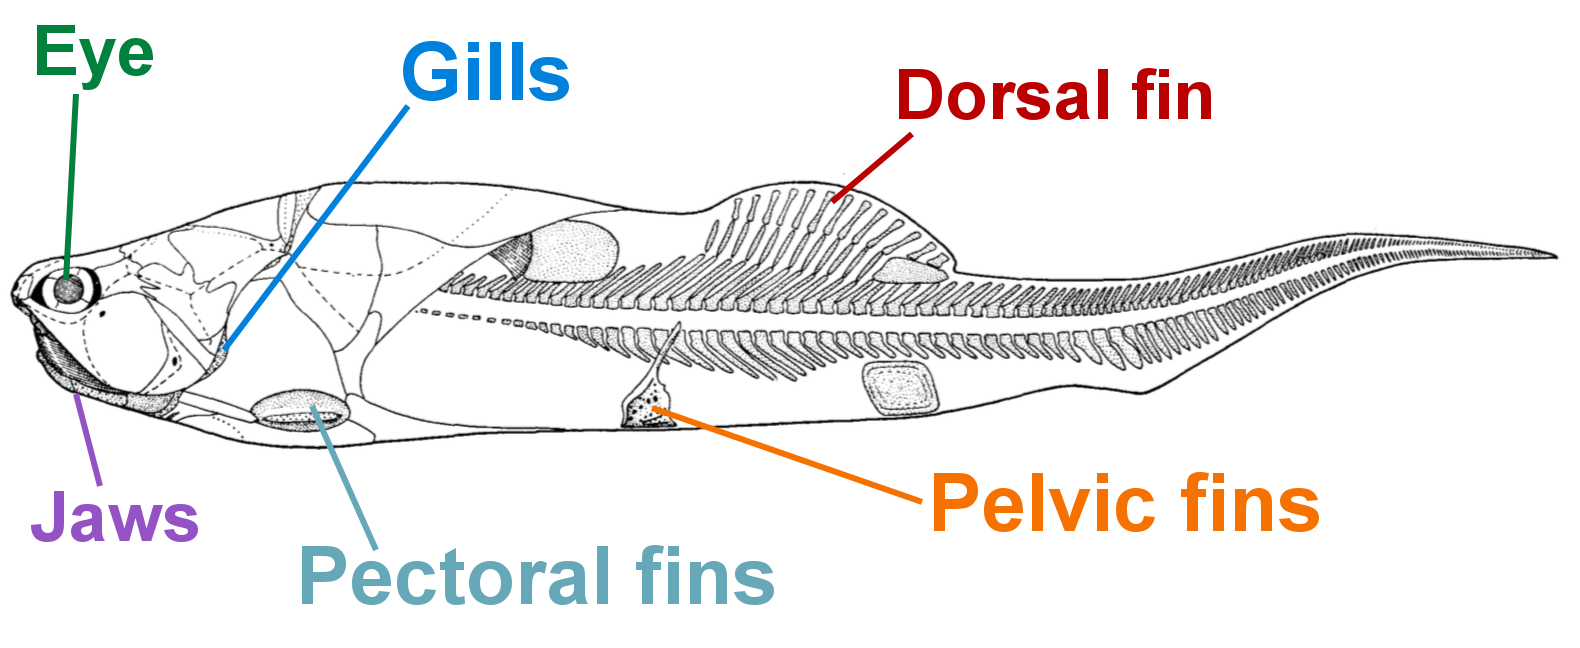
\includegraphics[scale=0.5]{Coccosteus}
\centering
\end{figure}

{\large\textbf{\underline{Fossil facts}}\par}

\begin{itemize}
\item While \textit{Coccosteus} itself wasn't all that big, some of its relatives could grow to enormous sizes.  One, \textit{Dunkleosteus}, was up to 6 metres long!
  \item One of the most obvious parts of our \textit{Coccosteus} is its backbone.  This tells us that it is a vertebrate.
\end{itemize}


\end{document}